% !BIB TS-program = biber
\documentclass[12pt]{article}
\usepackage{nameref}
\usepackage{amsmath}
\usepackage{graphicx}
\usepackage[margin=2cm]{geometry}
\usepackage[style=authoryear]{biblatex}
\addbibresource{main.bib}

\title{the title of the document}
\author{Jesse Knight}
\date{today}

\begin{document}
\maketitle

\section{Introduction}
In section \ref{s:methods} \nameref{s:methods},
we have the methods \parencite{Knight2019}.
In the work by \citeauthor{Knight2019} (\citeyear{Knight2019}),
we see

\section{Methods}\label{s:methods}
This is inline math: $x = 1$.
Equation (\ref{eq:math}) is not.
\begin{equation}
  \begin{aligned}
    e &= mc^2\\
    b &= mc^3 + \alpha\\
    d &= mc^4 + \beta + \gamma
    \label{eq:math}
  \end{aligned}
\end{equation}

\begin{equation}
  x(t) = \sum_{i=0}^{t} \left[\frac{1}{2}\right] A(\tau) d\tau
\end{equation}


\subsection{Experiment 1}
\subsection{Experiment 2}

\clearpage
\section{Results}

\begin{figure}[h]
    \centering
    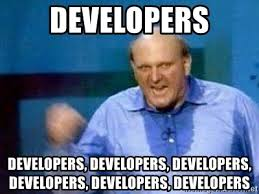
\includegraphics[width=0.5\linewidth]{download.jpg}%
    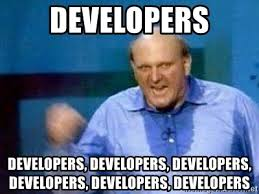
\includegraphics[width=0.5\linewidth]{download.jpg}
    \caption{Caption}
    \label{fig:my_label}
\end{figure}
\begin{table}[h]
    \centering
    \begin{tabular}{cc}
        a & b\\
        1 & 2
    \end{tabular}
    \caption{Caption}
    \label{tab:my_label}
\end{table}


\printbibliography

\end{document}